\documentclass[a4paper,12pt]{article}
\usepackage[top=2.5cm,bottom=2.5cm,left=2.5cm,right=2.5cm]{geometry}
%% \usepackage[brazil,brazilian]{babel}
\usepackage{amsmath, nccmath}
\usepackage{amsfonts}
\usepackage{amssymb}
\usepackage{multirow}
\usepackage{natbib}
\usepackage[colorlinks,citecolor=blue,urlcolor=blue]{hyperref}
\usepackage[utf8]{inputenc}
\usepackage{graphicx}  
\usepackage{float}
\usepackage{pdflscape} % horizontal page
\usepackage{tabularx}
\usepackage[english,vlined,ruled]{algorithm2e}
\usepackage{booktabs}
\usepackage{tikz}
\usetikzlibrary{positioning,shapes,arrows}
\usepackage{adjustbox}
\usepackage{tikz}
\usetikzlibrary{backgrounds}
\usetikzlibrary{arrows}
\usetikzlibrary{shapes,shapes.geometric,shapes.misc}

% this style is applied by default to any tikzpicture included via \tikzfig
\tikzstyle{tikzfig}=[baseline=-0.25em,scale=0.5]

% these are dummy properties used by TikZiT, but ignored by LaTex
\pgfkeys{/tikz/tikzit fill/.initial=0}
\pgfkeys{/tikz/tikzit draw/.initial=0}
\pgfkeys{/tikz/tikzit shape/.initial=0}
\pgfkeys{/tikz/tikzit category/.initial=0}

% standard layers used in .tikz files
\pgfdeclarelayer{edgelayer}
\pgfdeclarelayer{nodelayer}
\pgfsetlayers{background,edgelayer,nodelayer,main}

% style for blank nodes
\tikzstyle{none}=[inner sep=0mm]

% include a .tikz file
\newcommand{\tikzfig}[1]{%
{\tikzstyle{every picture}=[tikzfig]
\IfFileExists{#1.tikz}
  {\input{#1.tikz}}
  {%
    \IfFileExists{./figures/#1.tikz}
      {\input{./figures/#1.tikz}}
      {\tikz[baseline=-0.5em]{\node[draw=red,font=\color{red},fill=red!10!white] {\textit{#1}};}}%
  }}%
}

% the same as \tikzfig, but in a {center} environment
\newcommand{\ctikzfig}[1]{%
\begin{center}\rm
  \tikzfig{#1}
\end{center}}

% fix strange self-loops, which are PGF/TikZ default
\tikzstyle{every loop}=[]


\title{
  
  Modeling the cumulative incidence function of clustered competing
  risks data: a multinomial GLMM approach

}
\author{
  Henrique Aparecido Laureano\thanks{
    Laboratory of Statistics and Goeinformation,
    Departament of Statistics,
    Paran\'{a} Federal University, Curitiba, Brazil.
    E-mail: laureano@ufpr.br
  }~
  Wagner Hugo Bonat$^\ast$}
 
\begin{document}
\maketitle

\begin{abstract}

  Clustered competing risks data are a complex failure time data
  scheme. Its main characteristics are the cluster structure, which
  implies a latent within-cluster dependence between its elements, and
  its multiple variables competing to be the one responsible for the
  occurrence of an event, the failure. To handle this kind of data, we
  propose a full likelihood approach, based on a generalized linear
  mixed model instead a usual complex frailty model. We model the
  competing causes in the probability scale, in terms of the cumulative
  incidence function (CIF). A multinomial distribution is assumed for
  the competing causes and censorship, conditioned on the latent
  effects. The latent effects are accommodated via a multivariate
  Gaussian distribution. The CIF is specified as the product of an
  instantaneous risk level function with a failure time trajectory level
  function. The estimation procedure is performed through the R package
  TMB (Template Model Builder), an \texttt{C++} based framework with
  efficient Laplace approximation and automatic differentiation
  routines. A large simulation study is performed, based on different
  latent structure formulations. The model presents to be of difficult
  estimation, with our results converging to a latent structure where
  the risk and failure time trajectory levels are correlated.

\end{abstract}

\begin{flushleft}
 \textbf{Keywords}: 
 Clustered competing risks;
 Within-cluster dependence;
 Multinomial generalized linear mixed model (GLMM);
 TMB: Template Model Builder;
 Laplace approximation;
 Automatic differentiation (AD).                    
\end{flushleft}

\section{Introduction}

Failure time data is the branch of Statistics responsible to handle
random variables describing the time until the occurrence of an event, a
failure \citep{kalb&prentice,hougaard00}. The time until a failure is
called survival experience, the modeling object. To accommodate the
number of possible causes for a failure and the way how they relate,
different failure time data layouts were proposed and are shown in
Figure \ref{fig:failuretimedata}. The first two are special cases of the
last, a multistate process. The special cases are characterized by the
presence of only absorbent states, besides the initial state 0. A
multistate process is characterized by the presence of at least one
intermediate state. In this work, our focus is on the competing risks
process, more specifically, its clustered version i.e., with groups of
elements sharing some non-observed latent dependence structure.

\begin{figure}[H]
 \centering
 \scalebox{0.85}{
  \begin{tikzpicture}
   \begin{pgfonlayer}{nodelayer}
    \node [style=circle,draw=black,fill=white] (2) at (-17.5, 5.5) {0};
    \node [style=circle,draw=black,fill=white] (3) at (-13.5, 5.5) {1};
    \node [style=circle,draw=black,fill=white] (7) at (-7.5, 5.5) {1};
    \node [style=circle,draw=black,fill=white] (9) at (-7.5, 4.5) {2};
    \node [style=none] (11) at (-7.5, 3.5) {$\vdots$};
    \node [style=circle,draw=black,fill=white] (12) at (-7.5, 2.5) {$m$};
    \node [style=circle,draw=black,fill=white] (14) at (-12.25, 4) {0};
    \node [style=circle,draw=black,fill=white] (22) at (-6, 3.5) {0};
    \node [style=circle,draw=black,fill=white] (23) at (-2, 3.5) {2};
    \node [style=circle,draw=black,fill=white] (25) at (-4, 5.5) {1};
    \node [style=none] (27) at (-17, 5.5) {};
    \node [style=none] (28) at (-14, 5.5) {};
    \node [style=none] (29) at (-11.75, 4.25) {};
    \node [style=none] (30) at (-8, 5.5) {};
    \node [style=none] (31) at (-8, 4.5) {};
    \node [style=none] (32) at (-8, 2.5) {};
    \node [style=none] (33) at (-5.5, 3.5) {};
    \node [style=none] (34) at (-4.5, 5.25) {};
    \node [style=none] (35) at (-2.5, 3.5) {};
    \node [style=none] (36) at (-11.75, 4) {};
    \node [style=none] (37) at (-11.75, 3.75) {};
    \node [style=none] (38) at (-5.5, 3.75) {};
    \node [style=none] (39) at (-2.5, 3.75) {};
    \node [style=none] (40) at (-3.5, 5.25) {};
    \node [style=none] (44) at (-15.5, 6.75) {{\large
                                               Failure time process}};
    \node [style=none] (45) at (-10, 6.75) {{\large
                                             Competing risks process}};
    \node [style=none] (47) at (-4, 6.75) {{\large Multistate process}};
   \end{pgfonlayer}
   \begin{pgfonlayer}{edgelayer}
	\draw [style=1side] (27.center) to (28.center);
	\draw [style=1side] (37.center) to (32.center);
	\draw [style=1side] (40.center) to (39.center);
	\draw [style=1side] (33.center) to (35.center);
	\draw [style=2side] (38.center) to (34.center);
	\draw [style=1side] (36.center) to (31.center);
	\draw [style=1side] (29.center) to (30.center);
   \end{pgfonlayer}
  \end{tikzpicture}
 }
 \caption{Illustration of failure time data layouts.}
 \label{fig:failuretimedata}
\end{figure}

In the analysis of failure time data, the survival experiences are
usually modeled in the hazard (failure rate) scale, and when the latent
within-cluster dependence is accommodated we have the so-called frailty
models \citep{frailty78,frailty79,liang95,petersen98,therneau00}. The
use of frailty models implies complicated likelihood functions and its
inference is done via elaborated and slow EM algorithms
\citep{nielsen92,klein92} or inefficient MCMC schemes
\citep{hougaard00}. Besides, its conclusions are attached to its
modeling scale i.e., all model interpretations are in terms of not
straightforward hazard rates.

A less usual scale is to model the survival experiences in the
probability scale.

The class of generalized linear models (GLMs) \citep{GLM72} is probably
the most popular statistical modelling framework. Despite its
flexibility, the GLMs are not suitable for dependent data. In the case
of longitudinal data, it is essential that the regression model take
into account the longitudinal and/or grouped data structure. According
to \cite{diggle02} longitudinal data are repeated measures evaluated on
the same subjects over time, that are potentially correlated. Dependent
data can also arises in studies with block designs, spatial and
multilevel data \citep{verbeke&molenberghs,fitzmaurice}. For the
analysis of such data several methods have been proposed over the last
four decades.

\cite{laird82} proposed the random effects regression models for
longitudinal data analysis. \cite{breslow93} presented the generalized
linear mixed models~(GLMMs) for the analysis of non-Gaussian
outcomes. \cite{gcmr} developed a class of marginal models for modelling
dependence structures in the analysis of longitudinal data, time series
and spatial based on Gaussian copula models.

The main goal of this study is to propose the . In this paper, we will
investigate the as an alternative to . R \citep{R21} package
\texttt{TMB} \citep{TMb}.

The main contributions of this article are: (i) introducing the unit
gamma distribution into the GLMMs framework; (ii) performing a extensive
simulation study to check the properties of the the maximum likelihood
estimator to deal with longitudinal continuous bounded outcomes; (iii)
applying the proposed model in two data sets from different fields of
application; (iv) providing R code and \texttt{C++} implementation for
the unit gamma mixed models.

The work are organized as follows. Section \ref{model}, Section
\ref{inference}, Section \ref{simulation}. Finally, the main
contributions of the article are discussed in Section \ref{discussion}.

\section{multiGLMM: a multinomial GLMM for clustered competing risks data}
\label{model}

\begin{figure}[H]
 \centering 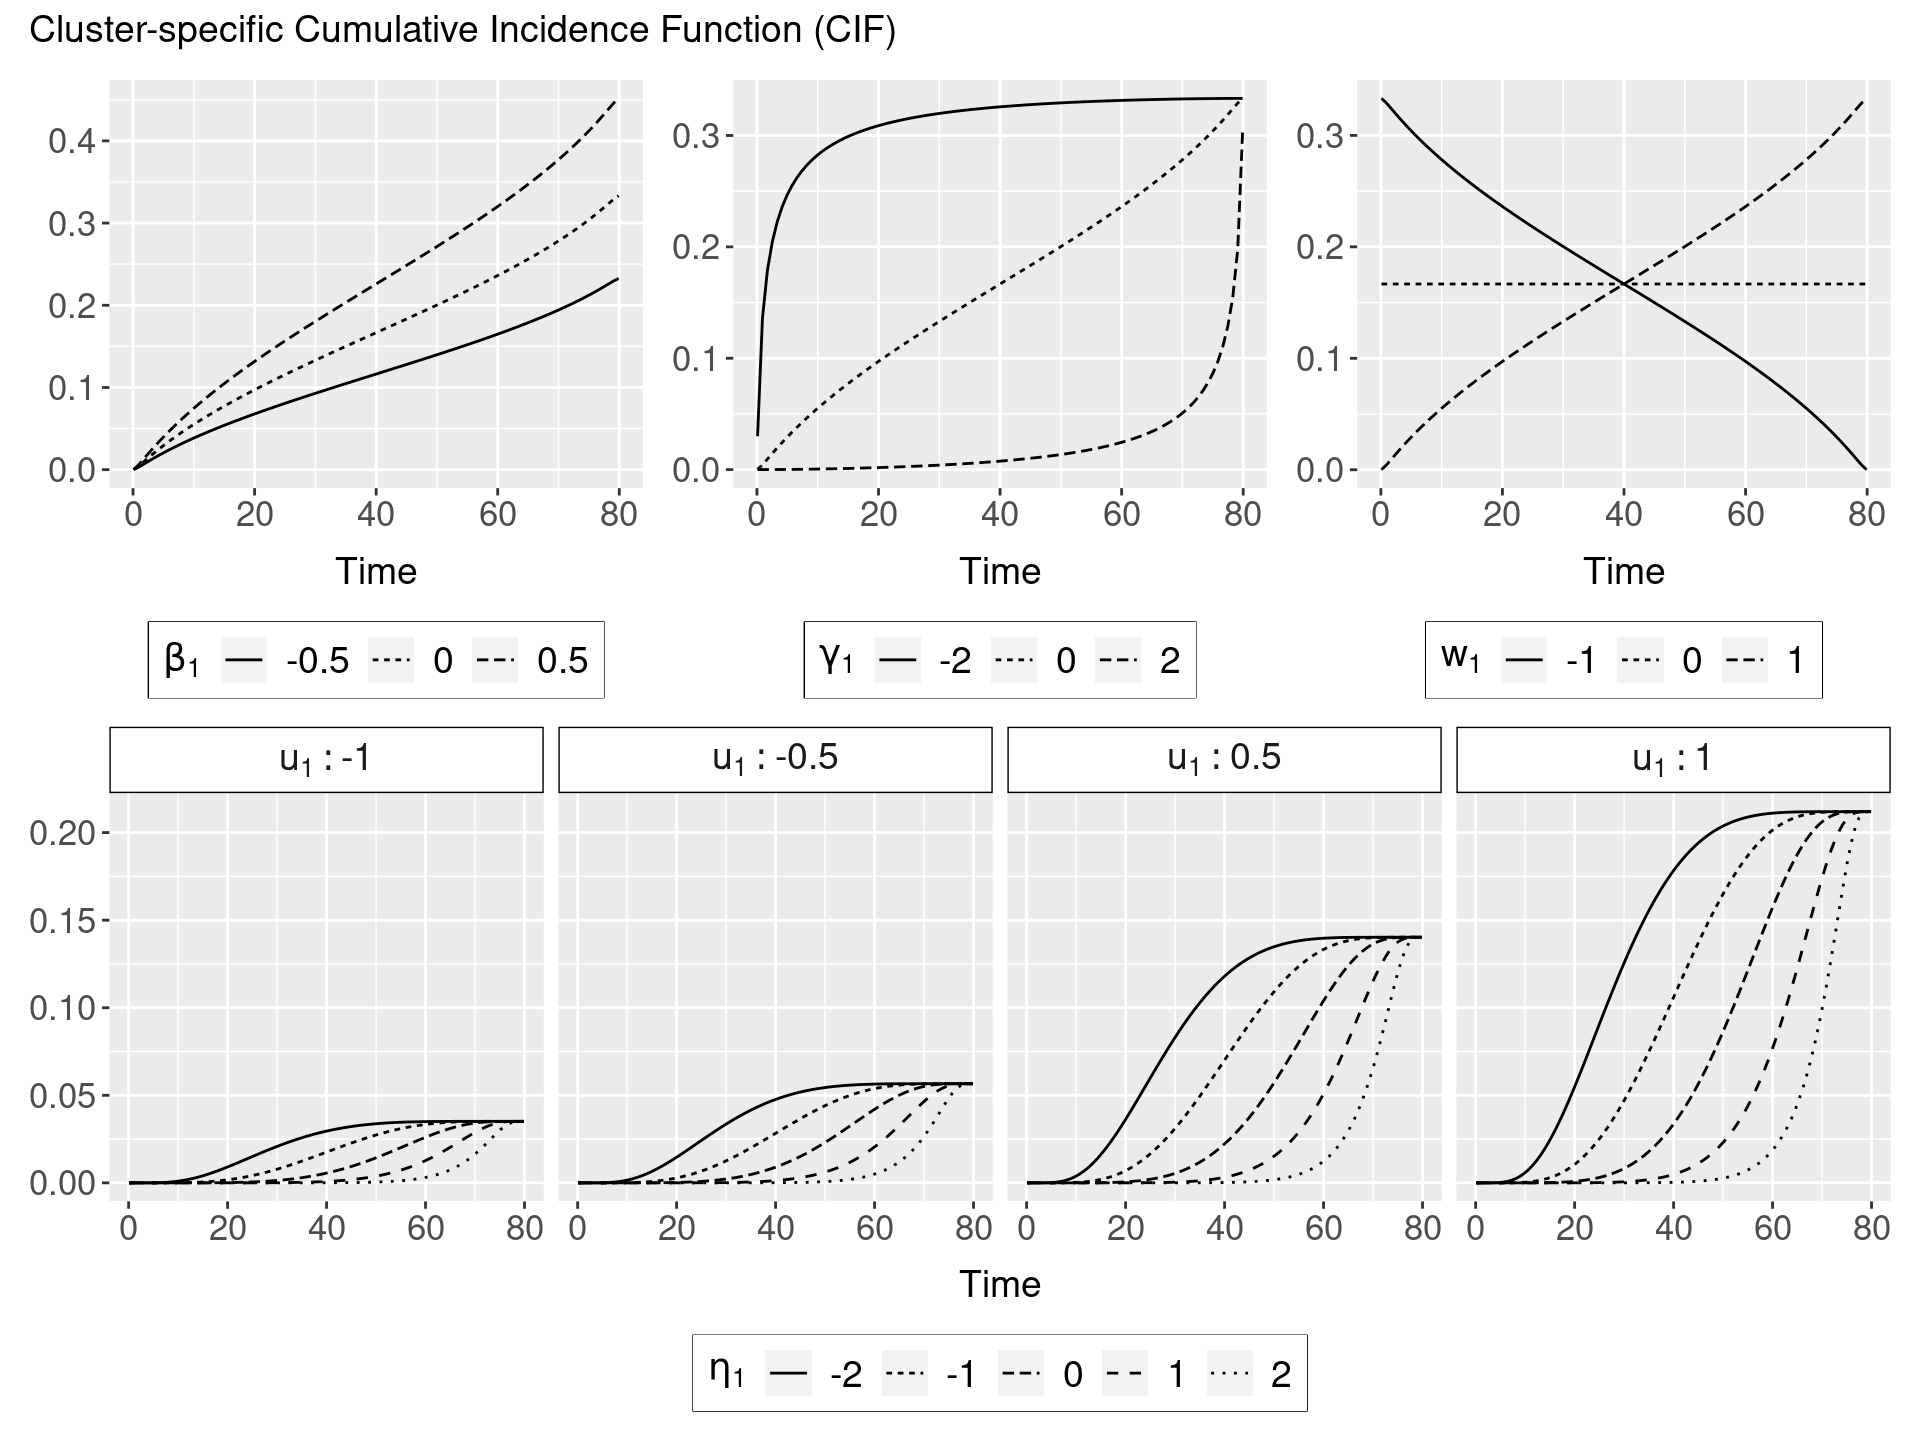
\includegraphics[width=\linewidth]{pics/cifstudy-1.png}
 \vspace{-0.75cm}
 \caption{Curve behaviors for different parameter settings, showing then
   the corresponding parameter effects in a cluster-specific cumulative
   incidence function (CIF).}
 \label{fig:cifcoefs}
\end{figure}

\section{Estimation and inference}
\label{inference}

\section{Simulation studies}
\label{simulation}

\section{Discussion}
\label{discussion}

\section*{Supplementary material}

\bibliographystyle{dcu}
\bibliography{references}

\end{document}
